% Options for packages loaded elsewhere
\PassOptionsToPackage{unicode}{hyperref}
\PassOptionsToPackage{hyphens}{url}
%
\documentclass[
  ignorenonframetext,
]{beamer}
\usepackage{pgfpages}
\setbeamertemplate{caption}[numbered]
\setbeamertemplate{caption label separator}{: }
\setbeamercolor{caption name}{fg=normal text.fg}
\beamertemplatenavigationsymbolsempty
% Prevent slide breaks in the middle of a paragraph
\widowpenalties 1 10000
\raggedbottom
\setbeamertemplate{part page}{
  \centering
  \begin{beamercolorbox}[sep=16pt,center]{part title}
    \usebeamerfont{part title}\insertpart\par
  \end{beamercolorbox}
}
\setbeamertemplate{section page}{
  \centering
  \begin{beamercolorbox}[sep=12pt,center]{part title}
    \usebeamerfont{section title}\insertsection\par
  \end{beamercolorbox}
}
\setbeamertemplate{subsection page}{
  \centering
  \begin{beamercolorbox}[sep=8pt,center]{part title}
    \usebeamerfont{subsection title}\insertsubsection\par
  \end{beamercolorbox}
}
\AtBeginPart{
  \frame{\partpage}
}
\AtBeginSection{
  \ifbibliography
  \else
    \frame{\sectionpage}
  \fi
}
\AtBeginSubsection{
  \frame{\subsectionpage}
}
\usepackage{lmodern}
\usepackage{amssymb,amsmath}
\usepackage{ifxetex,ifluatex}
\ifnum 0\ifxetex 1\fi\ifluatex 1\fi=0 % if pdftex
  \usepackage[T1]{fontenc}
  \usepackage[utf8]{inputenc}
  \usepackage{textcomp} % provide euro and other symbols
\else % if luatex or xetex
  \usepackage{unicode-math}
  \defaultfontfeatures{Scale=MatchLowercase}
  \defaultfontfeatures[\rmfamily]{Ligatures=TeX,Scale=1}
\fi
% Use upquote if available, for straight quotes in verbatim environments
\IfFileExists{upquote.sty}{\usepackage{upquote}}{}
\IfFileExists{microtype.sty}{% use microtype if available
  \usepackage[]{microtype}
  \UseMicrotypeSet[protrusion]{basicmath} % disable protrusion for tt fonts
}{}
\makeatletter
\@ifundefined{KOMAClassName}{% if non-KOMA class
  \IfFileExists{parskip.sty}{%
    \usepackage{parskip}
  }{% else
    \setlength{\parindent}{0pt}
    \setlength{\parskip}{6pt plus 2pt minus 1pt}}
}{% if KOMA class
  \KOMAoptions{parskip=half}}
\makeatother
\usepackage{xcolor}
\IfFileExists{xurl.sty}{\usepackage{xurl}}{} % add URL line breaks if available
\IfFileExists{bookmark.sty}{\usepackage{bookmark}}{\usepackage{hyperref}}
\hypersetup{
  pdftitle={Let's shine with Shiny (An Intro)},
  pdfauthor={Erika Siregar \textless@erikaris\textgreater{}},
  hidelinks,
  pdfcreator={LaTeX via pandoc}}
\urlstyle{same} % disable monospaced font for URLs
\newif\ifbibliography
\usepackage{color}
\usepackage{fancyvrb}
\newcommand{\VerbBar}{|}
\newcommand{\VERB}{\Verb[commandchars=\\\{\}]}
\DefineVerbatimEnvironment{Highlighting}{Verbatim}{commandchars=\\\{\}}
% Add ',fontsize=\small' for more characters per line
\usepackage{framed}
\definecolor{shadecolor}{RGB}{248,248,248}
\newenvironment{Shaded}{\begin{snugshade}}{\end{snugshade}}
\newcommand{\AlertTok}[1]{\textcolor[rgb]{0.94,0.16,0.16}{#1}}
\newcommand{\AnnotationTok}[1]{\textcolor[rgb]{0.56,0.35,0.01}{\textbf{\textit{#1}}}}
\newcommand{\AttributeTok}[1]{\textcolor[rgb]{0.77,0.63,0.00}{#1}}
\newcommand{\BaseNTok}[1]{\textcolor[rgb]{0.00,0.00,0.81}{#1}}
\newcommand{\BuiltInTok}[1]{#1}
\newcommand{\CharTok}[1]{\textcolor[rgb]{0.31,0.60,0.02}{#1}}
\newcommand{\CommentTok}[1]{\textcolor[rgb]{0.56,0.35,0.01}{\textit{#1}}}
\newcommand{\CommentVarTok}[1]{\textcolor[rgb]{0.56,0.35,0.01}{\textbf{\textit{#1}}}}
\newcommand{\ConstantTok}[1]{\textcolor[rgb]{0.00,0.00,0.00}{#1}}
\newcommand{\ControlFlowTok}[1]{\textcolor[rgb]{0.13,0.29,0.53}{\textbf{#1}}}
\newcommand{\DataTypeTok}[1]{\textcolor[rgb]{0.13,0.29,0.53}{#1}}
\newcommand{\DecValTok}[1]{\textcolor[rgb]{0.00,0.00,0.81}{#1}}
\newcommand{\DocumentationTok}[1]{\textcolor[rgb]{0.56,0.35,0.01}{\textbf{\textit{#1}}}}
\newcommand{\ErrorTok}[1]{\textcolor[rgb]{0.64,0.00,0.00}{\textbf{#1}}}
\newcommand{\ExtensionTok}[1]{#1}
\newcommand{\FloatTok}[1]{\textcolor[rgb]{0.00,0.00,0.81}{#1}}
\newcommand{\FunctionTok}[1]{\textcolor[rgb]{0.00,0.00,0.00}{#1}}
\newcommand{\ImportTok}[1]{#1}
\newcommand{\InformationTok}[1]{\textcolor[rgb]{0.56,0.35,0.01}{\textbf{\textit{#1}}}}
\newcommand{\KeywordTok}[1]{\textcolor[rgb]{0.13,0.29,0.53}{\textbf{#1}}}
\newcommand{\NormalTok}[1]{#1}
\newcommand{\OperatorTok}[1]{\textcolor[rgb]{0.81,0.36,0.00}{\textbf{#1}}}
\newcommand{\OtherTok}[1]{\textcolor[rgb]{0.56,0.35,0.01}{#1}}
\newcommand{\PreprocessorTok}[1]{\textcolor[rgb]{0.56,0.35,0.01}{\textit{#1}}}
\newcommand{\RegionMarkerTok}[1]{#1}
\newcommand{\SpecialCharTok}[1]{\textcolor[rgb]{0.00,0.00,0.00}{#1}}
\newcommand{\SpecialStringTok}[1]{\textcolor[rgb]{0.31,0.60,0.02}{#1}}
\newcommand{\StringTok}[1]{\textcolor[rgb]{0.31,0.60,0.02}{#1}}
\newcommand{\VariableTok}[1]{\textcolor[rgb]{0.00,0.00,0.00}{#1}}
\newcommand{\VerbatimStringTok}[1]{\textcolor[rgb]{0.31,0.60,0.02}{#1}}
\newcommand{\WarningTok}[1]{\textcolor[rgb]{0.56,0.35,0.01}{\textbf{\textit{#1}}}}
\usepackage{graphicx,grffile}
\makeatletter
\def\maxwidth{\ifdim\Gin@nat@width>\linewidth\linewidth\else\Gin@nat@width\fi}
\def\maxheight{\ifdim\Gin@nat@height>\textheight\textheight\else\Gin@nat@height\fi}
\makeatother
% Scale images if necessary, so that they will not overflow the page
% margins by default, and it is still possible to overwrite the defaults
% using explicit options in \includegraphics[width, height, ...]{}
\setkeys{Gin}{width=\maxwidth,height=\maxheight,keepaspectratio}
% Set default figure placement to htbp
\makeatletter
\def\fps@figure{htbp}
\makeatother
\setlength{\emergencystretch}{3em} % prevent overfull lines
\providecommand{\tightlist}{%
  \setlength{\itemsep}{0pt}\setlength{\parskip}{0pt}}
\setcounter{secnumdepth}{-\maxdimen} % remove section numbering

\title{Let's shine with Shiny (An Intro)}
\author{Erika Siregar
\href{https://twitter.com/erikaris}{\textless@erikaris\textgreater{}}}
\date{@RLadiesJakarta 6th Meetup --- February 2, 2020 Mozilla Community Space,
Jakarta}

\begin{document}
\frame{\titlepage}

\hypertarget{an-intro}{%
\section{An Intro}\label{an-intro}}

\begin{frame}{What is Shiny?}
\protect\hypertarget{what-is-shiny}{}

\begin{itemize}[<+->]
\tightlist
\item
  an \textbf{R package} for building an \textbf{interactive web apps}
  straight from R.
\item
  can be hosted as a \textbf{standalone} apps on a webpage ; or
  \textbf{embed} them in R Markdown documents ; or build
  \textbf{dashboards}.
\item
  can be extended with \textbf{CSS themes}, \textbf{htmlwidgets}, and
  \textbf{JavaScript actions}.
\end{itemize}

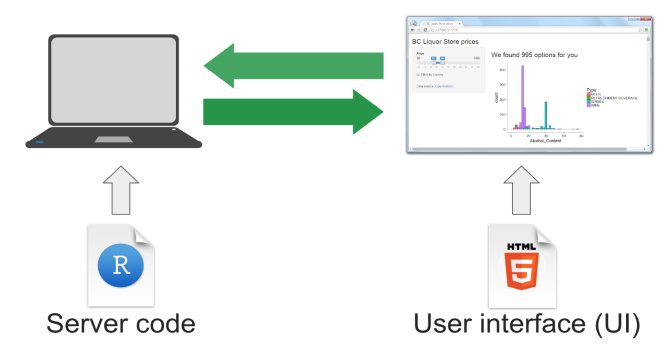
\includegraphics[width=1\textwidth,height=\textheight]{images/shiny.jpg}

\end{frame}

\begin{frame}{Why Shiny?}
\protect\hypertarget{why-shiny}{}

\begin{enumerate}[<+->]
\tightlist
\item
  Interactive
\item
  Animated
\end{enumerate}

\begin{figure}
\centering
\includegraphics{images/radar.gif}
\caption{\url{https://ceefluz.shinyapps.io/radar/}}
\end{figure}

\end{frame}

\hypertarget{enough-with-theory-lets-get-our-hands-dirty}{%
\section{Enough with Theory, Let's get our hands
dirty}\label{enough-with-theory-lets-get-our-hands-dirty}}

\begin{frame}[fragile]{4 Easy Steps to Build a Shiny App}
\protect\hypertarget{easy-steps-to-build-a-shiny-app}{}

\begin{enumerate}[<+->]
\item
  Load the Shiny library

\begin{Shaded}
\begin{Highlighting}[]
\KeywordTok{install.packages}\NormalTok{(}\StringTok{\textquotesingle{}shiny\textquotesingle{}}\NormalTok{)}
\KeywordTok{library}\NormalTok{(}\StringTok{\textquotesingle{}shiny\textquotesingle{}}\NormalTok{)}
\end{Highlighting}
\end{Shaded}
\item
  create the UI
\item
  create the server
\item
  combine the UI and server
\end{enumerate}

\begin{Shaded}
\begin{Highlighting}[]
\KeywordTok{library}\NormalTok{(shiny) }
\NormalTok{ui <{-}}\StringTok{ }\KeywordTok{fluidPage}\NormalTok{(...) }
\NormalTok{server <{-}}\StringTok{ }\ControlFlowTok{function}\NormalTok{(input, output, session) \{...\} }
\KeywordTok{shinyApp}\NormalTok{(}\DataTypeTok{ui =}\NormalTok{ ui, }\DataTypeTok{server =}\NormalTok{ server)}
\end{Highlighting}
\end{Shaded}

\end{frame}

\hypertarget{lets-walk-through-it}{%
\section{Let's walk through it}\label{lets-walk-through-it}}

\begin{frame}{Warming Up}
\protect\hypertarget{warming-up}{}

\begin{block}{a ``Hello, world'' Shiny app}

\begin{figure}
\centering
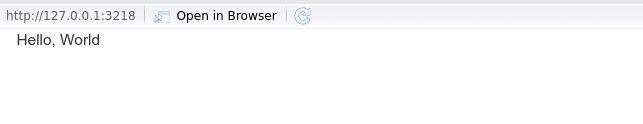
\includegraphics{images/hello_world2.jpg}
\caption{block1}
\end{figure}

\end{block}

\end{frame}

\begin{frame}{User Interface}
\protect\hypertarget{user-interface}{}

\textbf{Concept}: Input - Output - Render

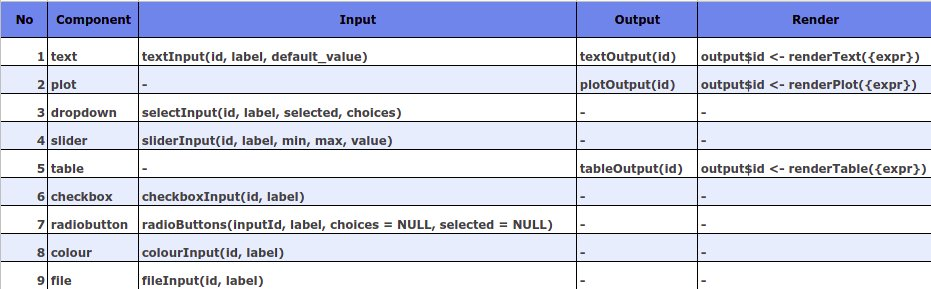
\includegraphics{images/component.jpg}

\end{frame}

\begin{frame}

See the complete list on
\href{https://github.com/rstudio/cheatsheets/raw/master/shiny.pdf}{Shiny
Cheatsheet}.

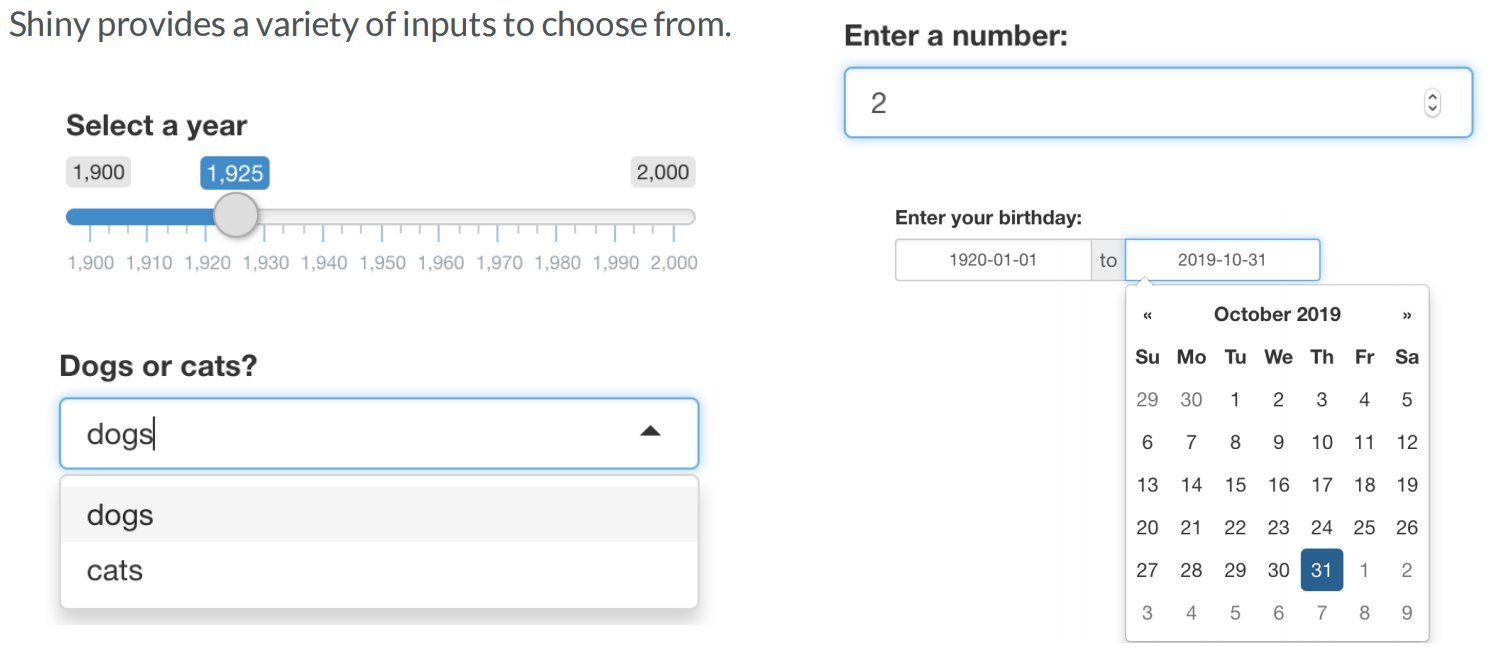
\includegraphics{images/inputs.jpg}

\end{frame}

\begin{frame}{TextInput}
\protect\hypertarget{textinput}{}

\begin{figure}
\centering
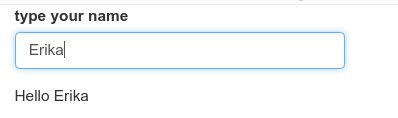
\includegraphics{images/textInput.jpg}
\caption{block2}
\end{figure}

\end{frame}

\begin{frame}{Adding Plot Container}
\protect\hypertarget{adding-plot-container}{}

\begin{figure}
\centering
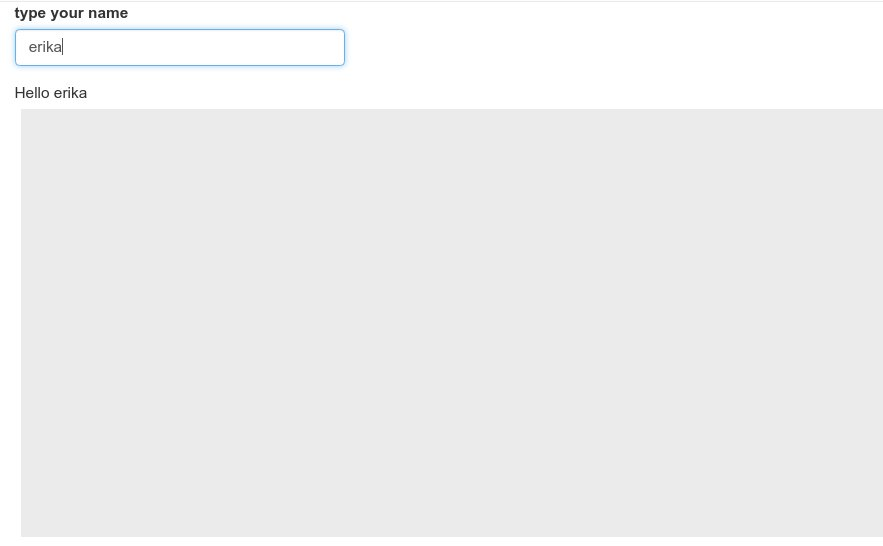
\includegraphics{images/plotContainer.jpg}
\caption{block3}
\end{figure}

\end{frame}

\begin{frame}{Layouting}
\protect\hypertarget{layouting}{}

\begin{figure}
\centering
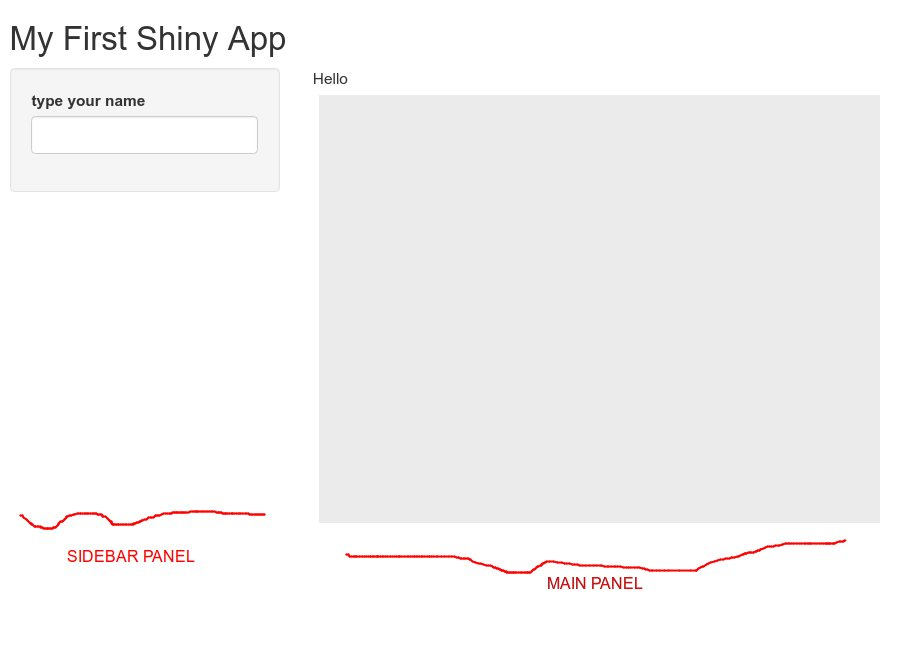
\includegraphics{images/layout.jpg}
\caption{block4}
\end{figure}

\end{frame}

\begin{frame}[fragile]{Let's Practice with Babynames}
\protect\hypertarget{lets-practice-with-babynames}{}

babynames is a package contains US Baby Names used for at least 5
children of either sex, from the year of 1880-2017.

\begin{Shaded}
\begin{Highlighting}[]
\KeywordTok{install.packages}\NormalTok{(}\StringTok{\textquotesingle{}babynames\textquotesingle{}}\NormalTok{)}
\KeywordTok{library}\NormalTok{(babynames)}
\end{Highlighting}
\end{Shaded}

\begin{figure}
\centering
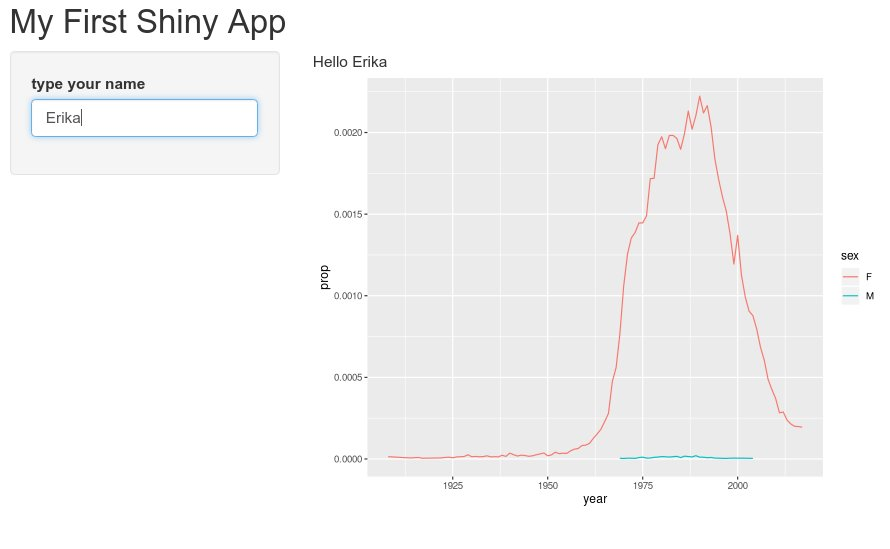
\includegraphics{images/babynames.jpg}
\caption{block5}
\end{figure}

\end{frame}

\begin{frame}{Select Input}
\protect\hypertarget{select-input}{}

\begin{figure}
\centering
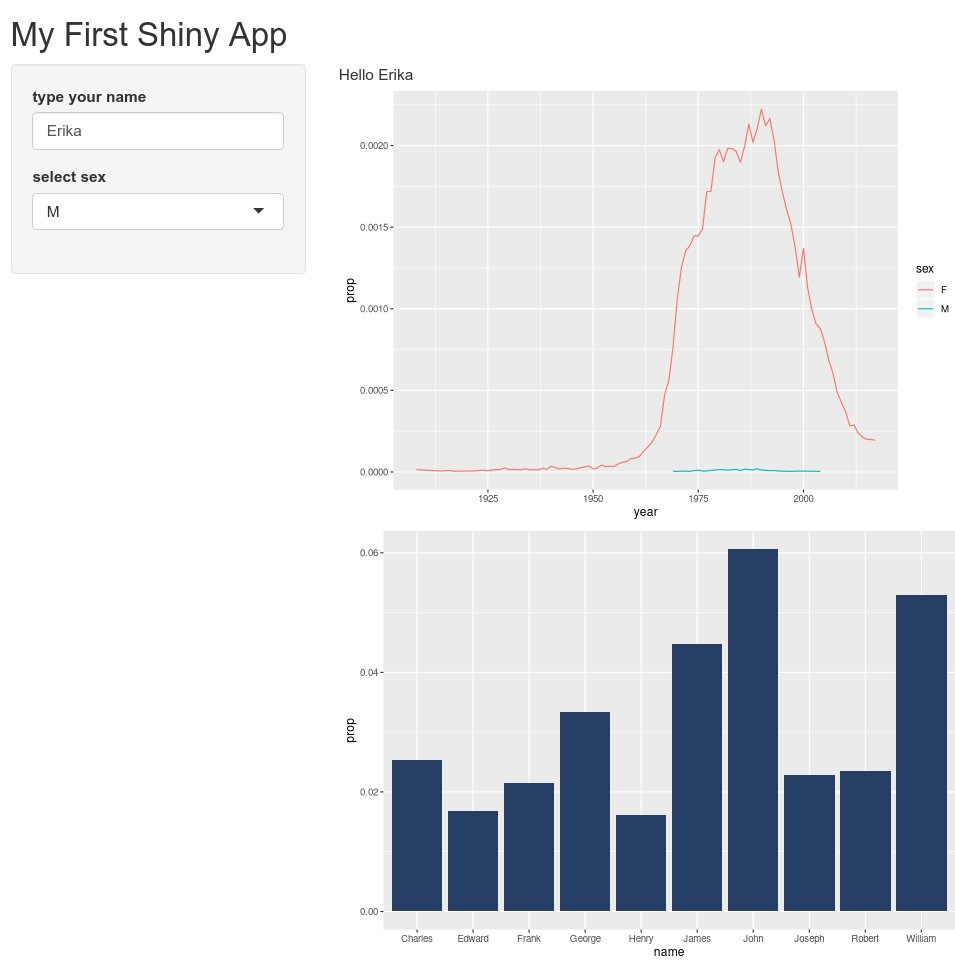
\includegraphics{images/select.jpg}
\caption{block6}
\end{figure}

\end{frame}

\begin{frame}{Slider}
\protect\hypertarget{slider}{}

\begin{figure}
\centering
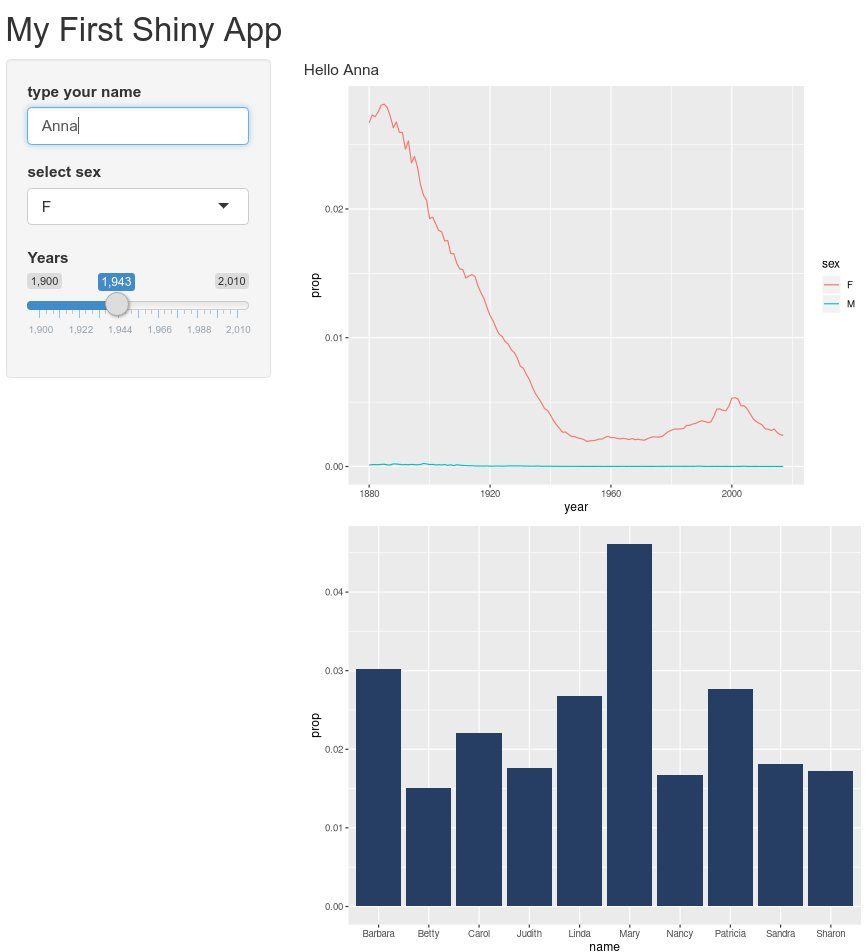
\includegraphics{images/slider.jpg}
\caption{block7}
\end{figure}

\end{frame}

\begin{frame}{tableOutput}
\protect\hypertarget{tableoutput}{}

\emph{Beware of the reactive variables}

\begin{figure}
\centering
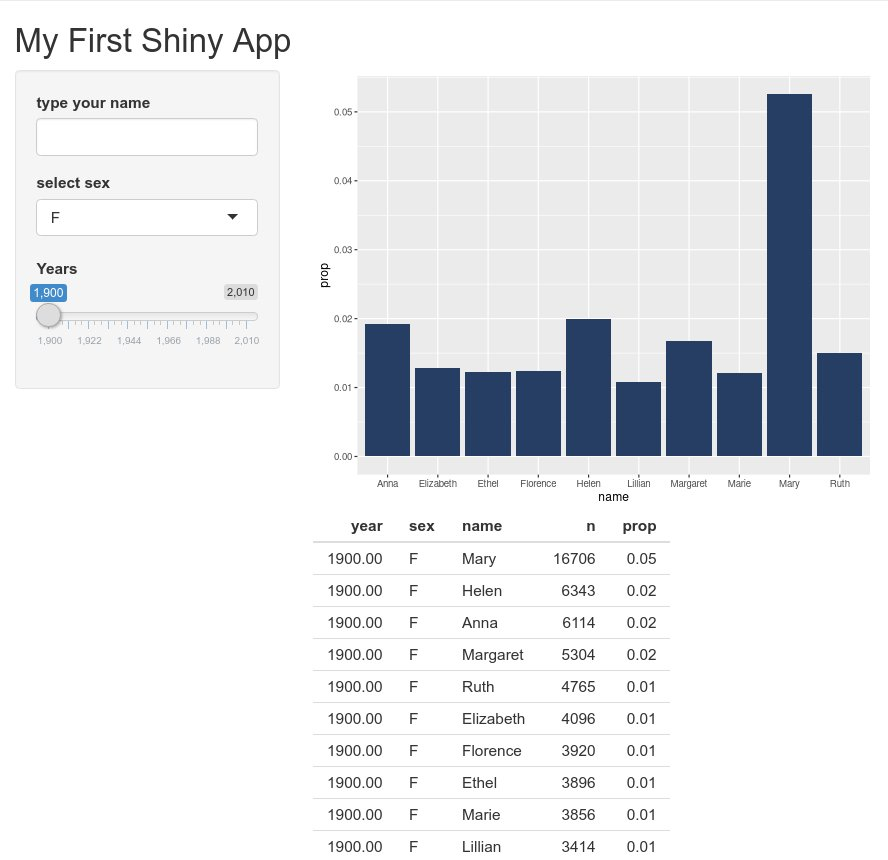
\includegraphics{images/table.jpg}
\caption{block8}
\end{figure}

\end{frame}

\begin{frame}[fragile]{Other option for Table}
\protect\hypertarget{other-option-for-table}{}

Using the package \texttt{DT}.

\begin{Shaded}
\begin{Highlighting}[]
  \KeywordTok{install.packages}\NormalTok{(}\StringTok{\textquotesingle{}DT\textquotesingle{}}\NormalTok{)}
  \KeywordTok{library}\NormalTok{(}\StringTok{\textquotesingle{}DT\textquotesingle{}}\NormalTok{)}
\end{Highlighting}
\end{Shaded}

\begin{figure}
\centering
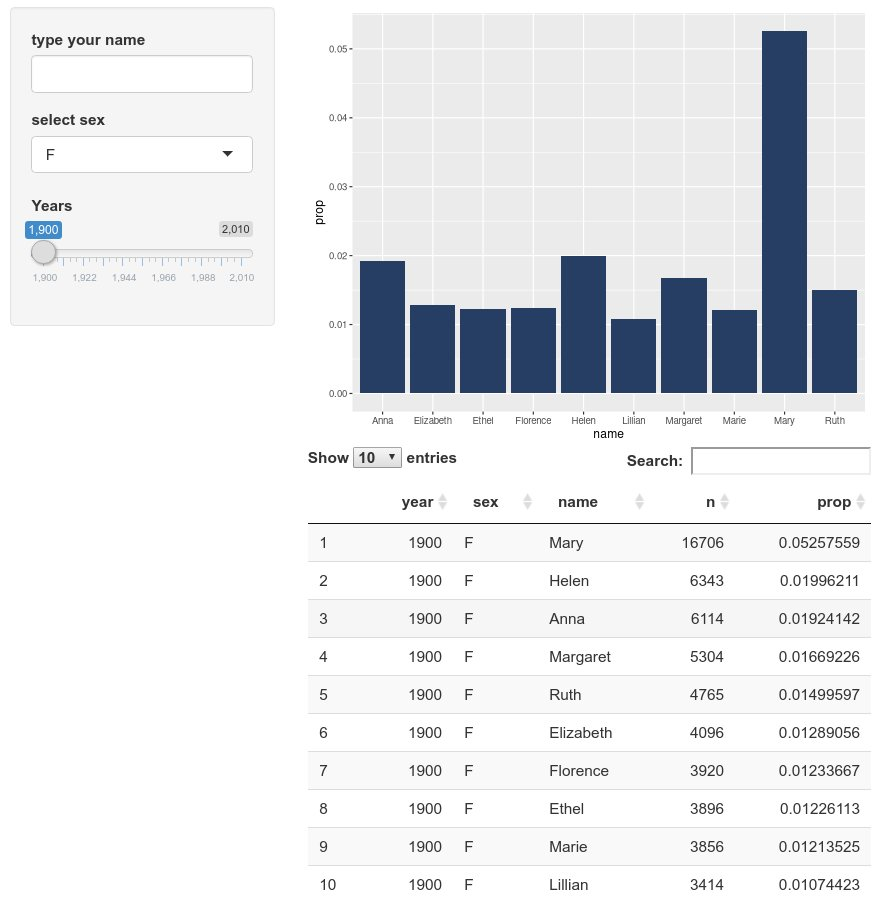
\includegraphics[width=0.6\textwidth,height=\textheight]{images/dttable.jpg}
\caption{block9}
\end{figure}

\end{frame}

\begin{frame}[fragile]{Interactive plot with plotly}
\protect\hypertarget{interactive-plot-with-plotly}{}

\begin{Shaded}
\begin{Highlighting}[]
  \KeywordTok{install.packages}\NormalTok{(}\StringTok{\textquotesingle{}plotly\textquotesingle{}}\NormalTok{)}
  \KeywordTok{library}\NormalTok{(}\StringTok{\textquotesingle{}plotly\textquotesingle{}}\NormalTok{)}
\end{Highlighting}
\end{Shaded}

\begin{figure}
\centering
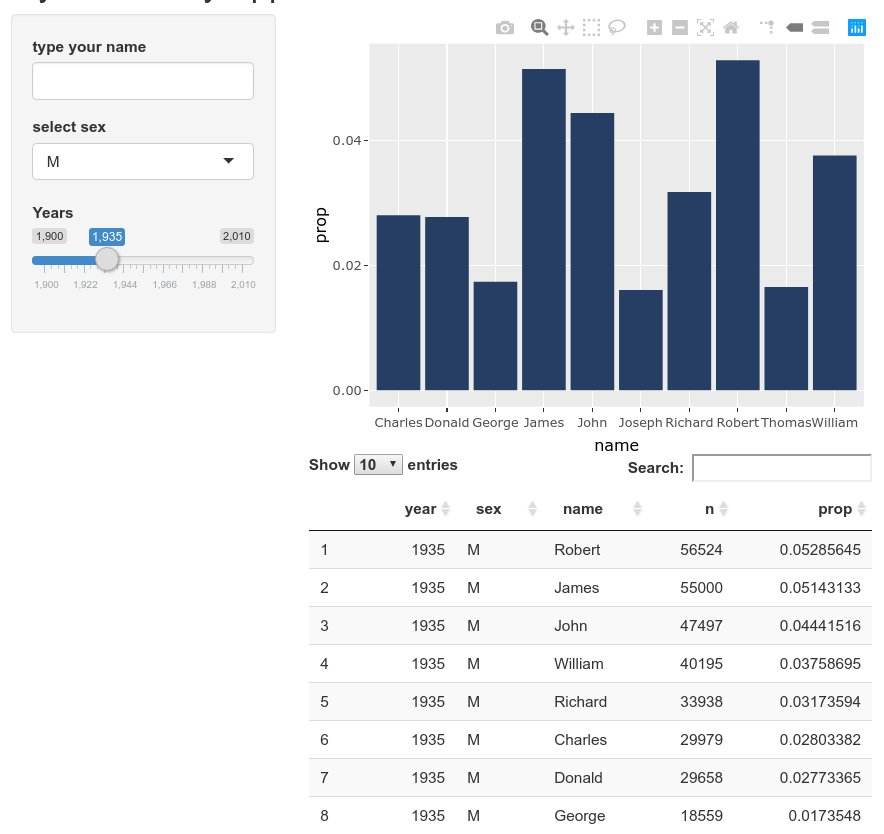
\includegraphics[width=0.6\textwidth,height=\textheight]{images/plotly.jpg}
\caption{block10}
\end{figure}

\end{frame}

\begin{frame}[fragile]{Working with Tabs}
\protect\hypertarget{working-with-tabs}{}

\begin{Shaded}
\begin{Highlighting}[]
\NormalTok{  ui <{-}}\StringTok{ }\KeywordTok{fluidPage}\NormalTok{(}
  \KeywordTok{sidebarLayout}\NormalTok{(}
    \KeywordTok{sidebarPanel}\NormalTok{(\_\_\_),}
    \KeywordTok{mainPanel}\NormalTok{(}
      \KeywordTok{tabsetPanel}\NormalTok{(}
        \KeywordTok{tabPanel}\NormalTok{(}\StringTok{"tab\_label\_1"}\NormalTok{ , \_\_\_),}
        \KeywordTok{tabPanel}\NormalTok{(}\StringTok{"tab\_label\_2"}\NormalTok{ , \_\_\_)}
\NormalTok{      ))))}
\end{Highlighting}
\end{Shaded}

\begin{figure}
\centering
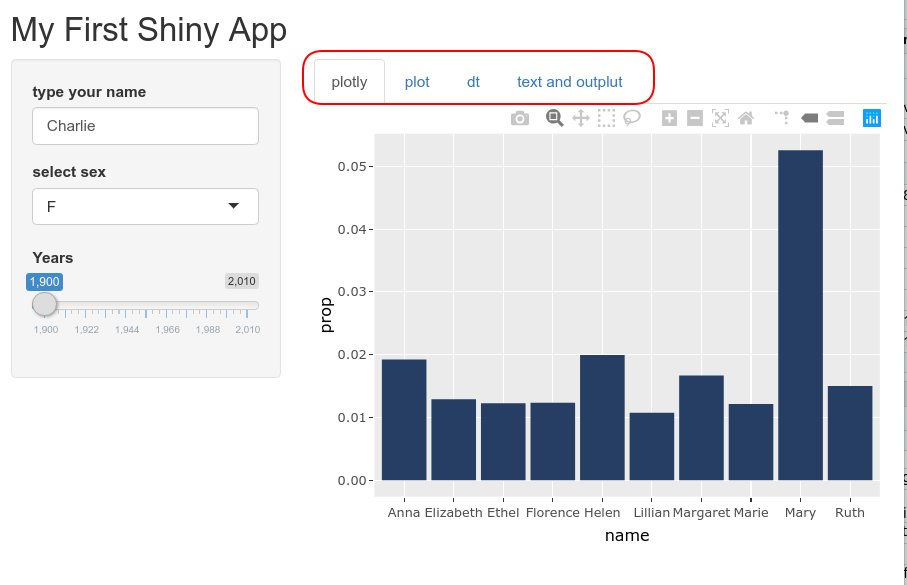
\includegraphics{images/tabs.jpg}
\caption{block11}
\end{figure}

\end{frame}

\begin{frame}[fragile]{Play with Themes}
\protect\hypertarget{play-with-themes}{}

\begin{Shaded}
\begin{Highlighting}[]
\KeywordTok{install.packages}\NormalTok{(}\StringTok{\textquotesingle{}shinythemes\textquotesingle{}}\NormalTok{)}
\KeywordTok{library}\NormalTok{(}\StringTok{\textquotesingle{}shinythemes\textquotesingle{}}\NormalTok{)}
\end{Highlighting}
\end{Shaded}

\begin{Shaded}
\begin{Highlighting}[]
\NormalTok{  shinythemes}\OperatorTok{::}\KeywordTok{themeSelector}\NormalTok{()  }\CommentTok{\# option 1}
\NormalTok{  theme =}\StringTok{ }\NormalTok{shinythemes}\OperatorTok{::}\KeywordTok{shinytheme}\NormalTok{(}\StringTok{\textquotesingle{}superhero\textquotesingle{}}\NormalTok{)  }\CommentTok{\# option 2}
\end{Highlighting}
\end{Shaded}

\begin{figure}
\centering
\includegraphics{images/themes.gif}
\caption{block12}
\end{figure}

\end{frame}

\begin{frame}{Bonus: Greeting Card}
\protect\hypertarget{bonus-greeting-card}{}

\begin{figure}
\centering
\includegraphics{images/greeting.gif}
\caption{block13}
\end{figure}

\end{frame}

\hypertarget{wrapup}{%
\section{Wrapup}\label{wrapup}}

\begin{frame}{Learn yourself}
\protect\hypertarget{learn-yourself}{}

\begin{enumerate}[<+->]
\tightlist
\item
  \url{https://shiny.rstudio.com/gallery/}
\item
  \url{https://github.com/rstudio/shiny-examples}
\end{enumerate}

\end{frame}

\begin{frame}{Any questions?}
\protect\hypertarget{any-questions}{}

Don't forget to follow Twitter: @RLadiesJakarta.

All materials are available on GitHub:
\url{https://github.com/rladiesjakarta}

\end{frame}

\end{document}
